\documentclass[hidelinks, 12pt, a4paper, brazil, oneside]{abntex2}

\usepackage[utf8]{inputenc}
\usepackage[brazil]{babel}
\usepackage[alf]{abntex2cite}
\usepackage{indentfirst}
\usepackage{graphicx}
\usepackage{float}
\usepackage{hyperref}

\titulo{Monitoramento em Conservadoras de Vacinas}
\autor{
    Alexandre Noronha \\
    Ezequiel Abreu \\
    Paulo Renato \\
    Pedro Esteves \\
}
\orientador{Rubem Cândido Santos}
\instituicao{Senai Centro}
\local{Belo Horizonte, Minas Gerais}
\data{2020}
\preambulo{
    Trabalho de conclusão de curso referente 
    ao segundo módulo do Técnico de Informatica para Internet, 
    requisito para o diploma do mesmo.
}

\begin{document}

\imprimircapa
\imprimirfolhaderosto

\listoffigures
\tableofcontents

\textual

\chapter{Introdução}

    A empresa 
    Rio Branco Alimentos SA/Fábrica de Rações de Patrocínio
    enfrenta um problema relacionado a falta de monitoramento 
    adequado da temperatura dos freezeres que guardam as vacinas
    da empresa.

    \begin{citacao}
        Atualmente temos 5 unidades de conservadoras de vacinas contendo 
        em média 30.000 doses cada uma.
        No passado tivemos problemas com perca de vacinas devido 
        defeito em uma das conservadoras levando a um prejuízo financeiro.
        Hoje não temos sistema de monitoramento automatizado ou meios 
        que garantam a conservação da vacina com a 
        manutenção da temperatura ideal. \cite{senaiDemanda}
    \end{citacao}

    Com o propósito de sanar esse problema decidiu-se por desenvolver
    um sistema para o gerenciamento da temperatura dos freezeres
    de cada unidade, de forma a aumentar a qualidade dos produtos
    entregues aos consumidores.

    Em relação a parte física do projeto consiste basicamente
    em instalar sensores de temperatura em cada freezer e 
    também instalar um sensor na porta para detectar se a 
    mesma esta aberta ou fechada. E cada sensor deverá transmitir 
    em tempo real os dados para um servidor e dessa forma 
    criar um histórico de variação de temperatura podendo 
    ser acessível quando necessário.

    Já sobre a parte do software o mesmo deve ter uma tela para
    poder cadastrar, atualizar e excluir os sensores do sistema, 
    e outra para visualização do histórico de temperatura e 
    e das variações em tempo real, mostrando se a porta esta 
    aberta ou fechada e emitindo um alerta caso a temperatura
    saia do nível especificado.

    A seleção da demanda foi feita através do portal Saga Senai, um 
    site onde empresas podem cadastrar seus problemas ou 
    dificuldades e os alunos do SENAI podem tentar resolver 
    esses problemas de forma inovadora. 
    Com isso os autores desse trabalho da turma TII2004M
    do curso de Informática para Internet do segundo modulo
    decidiram se desafiar a idealizar 
    uma solução estratégica inovadora para a situação 
    proposta pela empresa 
    Rio Branco Alimentos SA/Fábrica de Rações de Patrocínio.

    % Para o desenvolvimento desse projeto foi escolhido no 
    % Portal Saga Senai a demanda de
    % \href{http://plataforma.gpinovacao.senai.br/plataforma/demandas-da-industria/interna/4804}{monitoramento e conservação de vacinas}
    % onde a empresa tem uma dificuldade em monitorar a temperatura 
    % dos freezeres, para poder manter as vacinas em bom estado 
    % e assim evitar possíveis perdas.

\chapter{Objetivos}

    \section{Objetivo geral}

    Durante o desenvolvimento do projeto, 
    nosso principal objetivo
    % foi passar na matéria
    foi sanar da forma mais simples e eficaz 
    o problema da falta de monitoramento da 
    temperatura dos freezeres, e com isso poder 
    otimizar, facilitar e agregar mais valor 
    ao processo, como ao produto, 
    promovendo assim uma melhoria e facilidade 
    no controle de qualidade das vacinas que serão
    aplicadas.

    Através das mudanças e implementações 
    será possível adquirir uma maior qualidade das 
    vacinas, aumentar a confiabilidade no 
    gerenciamento de temperatura, eliminando
    ou reduzindo a necessidade de inspeções visuais 
    por parte dos funcionários, assim reduzindo 
    custos e perda dos produtos por temperaturas
    fora do esperado.

    % Para obter os resultados acima propomos 
    % a instalação de sensores no local de conservação 
    % das vacinas, possibilitando um monitoramento 
    % mais preciso e assertivo, em conjunto com a transmissão
    % em tempo real dos dados, permitirá aos funcionários 
    % e gestores se manterem informados a todo momento 
    % e tomar medidas rápidas caso algum imprevisto 
    % aconteça.

    \section{Objetivo especifico}
    Implementar os freezeres de conservação de vacinas 
    sensores de temperatura e integra-los a um banco de 
    dados juntamente com um sistema web capaz de gerenciar-los
    e suas respectivas temperaturas e 
    obter informações em tempo real sobre o status 
    de conservação das vacinas.

\chapter{Mapa Empático}

    A persona escolhida para criar o mapa empático
    foi a de Fernando, ele tem 37 anos e é o responsável
    pelo armazenamento e monitoramento das vacinas
    nas 5 unidades que a empresa 
    Rio Branco Alimentos SA/Fábrica de Rações de Patrocínio possui.

    Como podemos ver na figura \ref{fig:mapaEmpatico}
    o Fernando esta enfrenando um grave problema na 
    conservação das vacinas de sua empresa.
    No passado já perdeu parte do estoque para esse problema 
    e tem receio que isso volte a acontecer e perder ainda 
    mais produtos, invertimentos e elevar o custo
    e por consequência a credibilidade da 
    empresa perante o mercado.

    Fernando busca uma solução para essa demanda 
    como forma de garantir a qualidade das vacinas e
    manter a credibilidade da empresa e sanar as
    oscilações com relação ao gerenciamento da temperatura
    em todas as unidades.

    \begin{figure}
        \caption{Mapa empático}
        \centering
        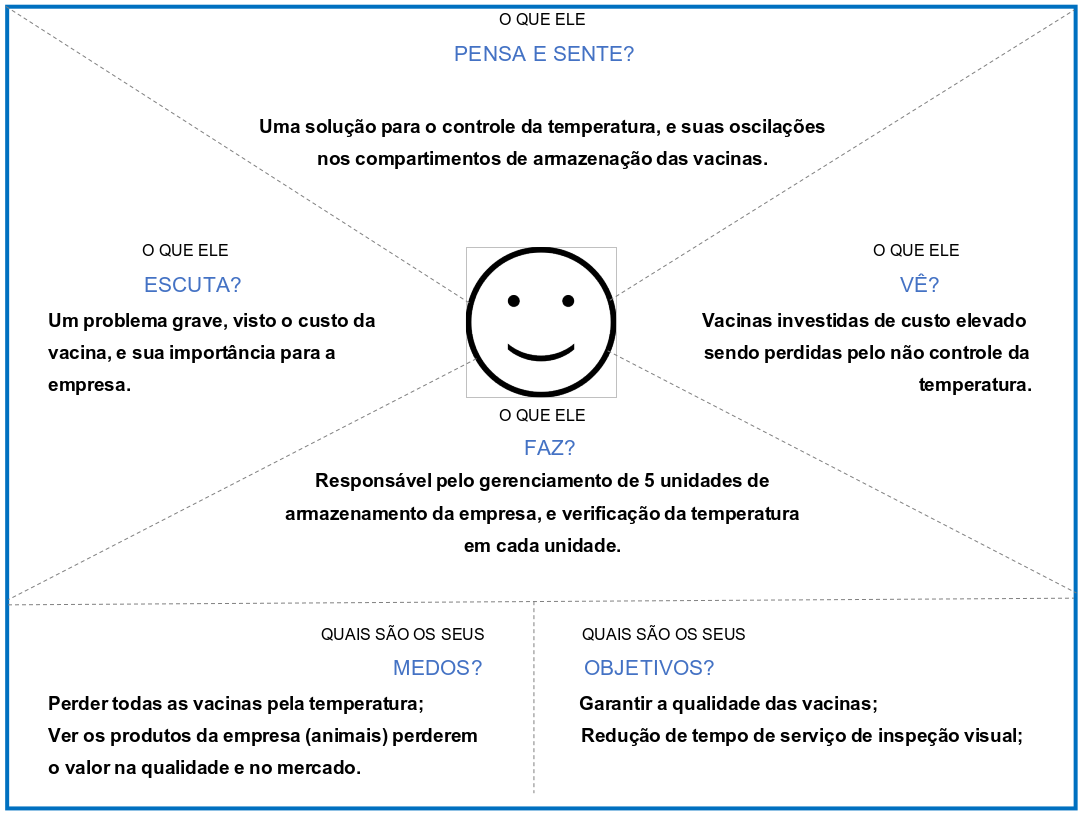
\includegraphics[width=0.85\textwidth]{img/mapa_empatico.png}
        \legend{Fonte: Elaborado pelos autores}
        \label{fig:mapaEmpatico}
    \end{figure}

\chapter{Desenvolvimento do projeto}

    O desenvolvimento do projeto foi dividido 
    em duas partes: a infraestrutura onde
    será tratado da parte física do projeto 
    necessária para o funcionamento 
    e o software que trata da parte de inteligencia
    do sistema e do histórico de variação de temperatura.

    De forma geral o funcionamento do projeto consiste
    como mostrado na figura \ref{fig:esquemaGeral}
    em sensores colocados em cada freezer e ligados 
    a um microcontrolador que estará conectado a internet
    e irá transmitir os dados de temperatura de cada 
    freezer para um servidor na nuvem, dados estes que poderão
    ser acessados através de um sistema web pelo computador
    ou um aplicativo (opcional) pelo celular.

    \begin{figure}[ht]
        \caption{Esquema Geral}
        \centering
        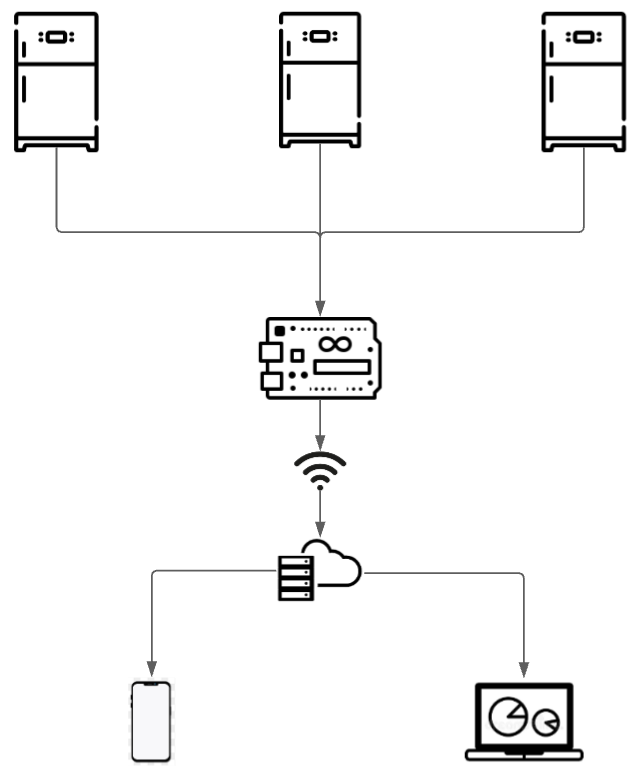
\includegraphics[width=0.5\textwidth]{img/esquema_geral.png}
        \legend{Fonte: Elaborado pelos autores}
        \label{fig:esquemaGeral}
    \end{figure}

\section{Infraestrutura}

    Quanto a infraestrutura será necessário um 
    investimento para possibilitar o monitoramento
    e garantir a segurança do sistema.

    Para ser possível verificar a temperatura atual do 
    freezer obviamente será imprescindível um termômetro,
    para ser mais especifico um sensor como uma sonda para facilitar
    o processo de instalação, que será integrado
    a um microcontrolador, como um CLP ou arduíno, 
    como mostrado na figura \ref{fig:termometro}.

    Para a escolha do termômetro o critério usado foi 
    a variação de temperatura, como especificado na demanda
    ``vacinas que devem ser conservadas a uma temperatura entre 2º à 8º C.''
    \citeonline{senaiDemanda},
    dito isso, como a variação de temperatura é pequena se faz 
    importante que o sensor tenha uma boa precisão ao 
    invés de suportar uma grande variação de temperatura.

    \begin{figure}[h]
        \caption{Sensor de temperatura}
        \centering
        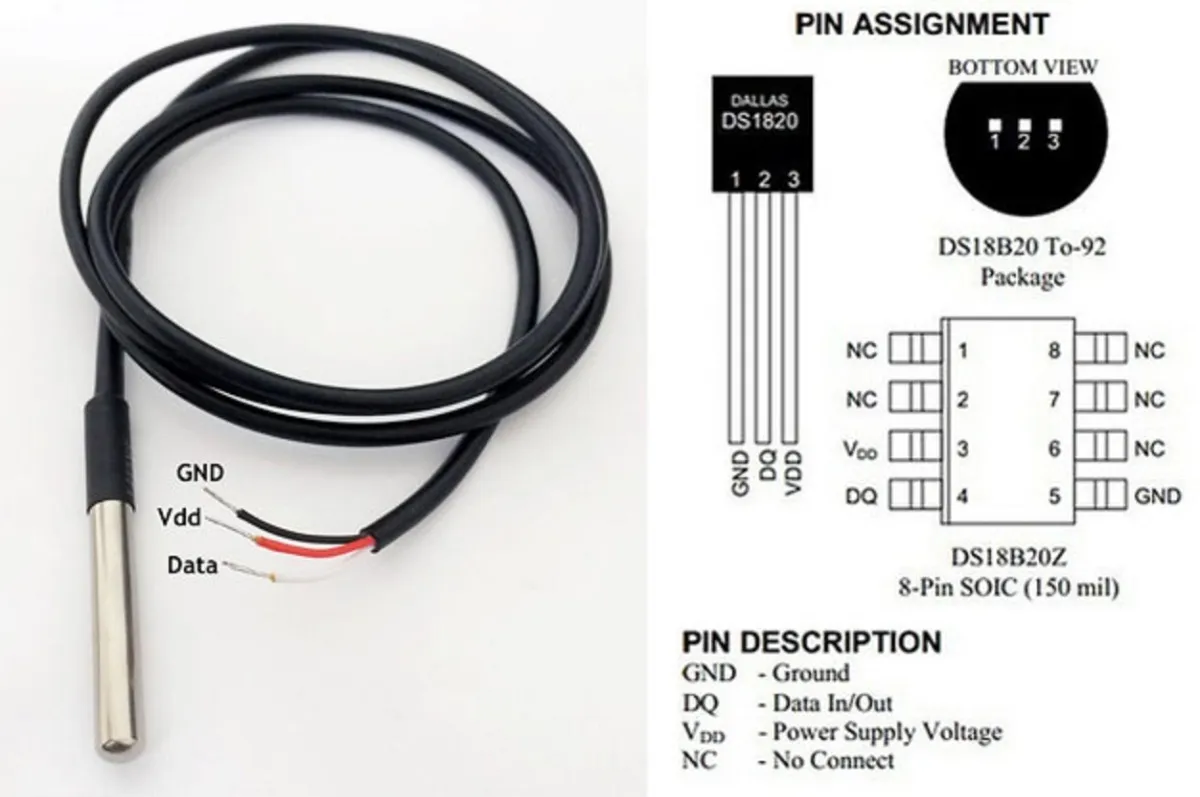
\includegraphics[width=0.8\textwidth]{img/termometro_esquema.png}
        \legend{Fonte: Retirado do site Mercado Livre \protect\footnotemark}
        \label{fig:termometro}
    \end{figure}

    \footnotetext{
        Disponível em: \url{https://produto.mercadolivre.com.br/MLB-1685461701}.
        Acesso em: 14 dez. 2020
    }

    Como o sensor térmico precisa ser ligado a um microcontrolador
    para poder transmitir a um servidor, pensando na segurança e 
    confiabilidade do sistema cada freezer deve ter seu próprio 
    microcontrolador para que na ocorrência de algum imprevisto
    isso possa ser facilmente isolado e corrigido sem afetar 
    outras partes do sistema.

    Considerando que cada freezer terá seu próprio microcontrolador
    facilitará assim a compra da peça pois cada microcontrolador 
    terá apenas a entrada do termômetro e do sensor de porta aberta;
    como saída um modulo de internet, uma lampada e uma sirene, 
    devido a esta quantidade de entradas e saídas pequena o custo
    de cada microcontrolador pode cair consideravelmente.

    \begin{figure}[ht]
        \caption{Arduíno Uno}
        \centering
        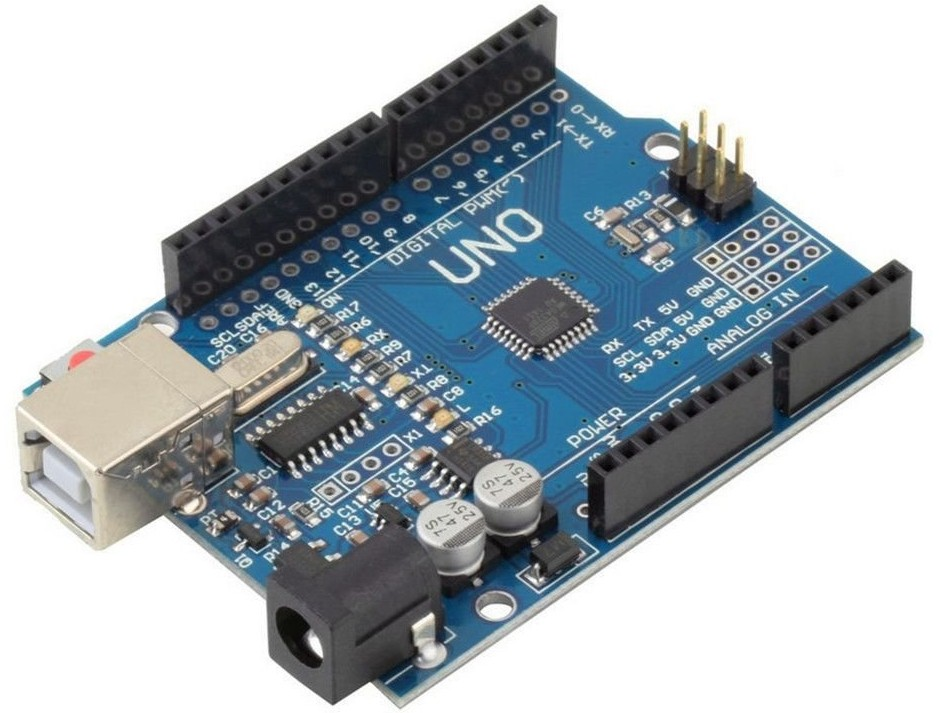
\includegraphics[width=0.85\textwidth]{img/arduino_uno.jpg}
        \legend{Fonte: Imagem retirada do site Eletrogate
            \protect\footnotemark
        }
        \label{fig:arduinoUno}
    \end{figure}

    \footnotetext{
        Disponível em: \url{https://www.eletrogate.com/uno-r3-smd-ch340-cabo-usb-para-arduino}.
        \\
        Acessado em 15 de Dez. 2020
    }

    Assim como mostrado na figura \ref{fig:arduinoUno}
    o microcontrolador escolhido é o arduíno Uno
    por ser simples, rápido, pequeno e de um baixo custo,
    este é muito usado em automação de processos
    de vários tipos. È recomendável para manter o 
    arduíno conservado e funcional coloca-lo em um case
    \footnote{
        Exemplo de case: \url{https://www.eletrogate.com/case-para-arduino-uno-em-acrilico-transparente}
        Acessado em 15 de Dez. 2020
    },
    uma caixa feita normalmente de plástico ou acrílico 
    para guardar e conservar-lo.

    Quanto ao servidor apesar de ser uma parte importante 
    da infraestrutura, pensando em manter a simplicidade 
    e segurança do sistema optamos por uma nuvem privada,
    como o Azure, AWS ou Google Cloud, no qual todos os 
    dados e infraestrutura é de responsabilidade da 
    nuvem contratada, sendo necessário investir apenas 
    em um bom link de internet para acessar os recursos 
    da nuvem.

    Sobre o link de internet para garantir a 
    alta disponibilidade do sistema tanto 
    para transmitir os dados dos sensores 
    como para visualizar e se manter atualizado
    no sistema web deve-se colocar um link redundante,
    assim a empresa não ficará presa a um único provedor 
    e em caso de alguma eventual falha o segundo link 
    assumirá mantendo tudo em funcionamento.


\section{Software (Sistema integrado)}

    Como dito anteriormente, os dados 
    dos sensores serão transmitidos para um banco de dados,
    nesse deverá ser gravado os dados dos sensores:
    as temperaturas minimas e máximas, também as temperaturas 
    padrão a cada 10 segundos, essa frequência de 
    escrita de temperatura no banco poderá ser alterado caso o 
    cliente assim deseje.

    Sobre a nuvem, ela deverá ser feita preferencialmente 
    em Kubernetes para poder facilmente gerenciar todos os containers 
    de cada parte da aplicação de forma isolada, e além disso 
    poder integrar e instalar o sistema em diferentes nuvens
    e alternar entre elas de forma simples e rápida, 
    proporcionando assim maior estabilidade e disponibilidade
    aos serviços do sistema.

    \begin{citacao}[english]
        (...)
        Kubernetes aims to simplify the deployment and management 
        of services, including the construction of applications 
        as sets of interacting but independent services.
        (...)
        \cite{brewer2015kubernetes}
    \end{citacao}

    Sobre as linguagens e ferramentas que serão utilizadas
    no sistema, o front-end será feito usando o framework 
    de JavaScript React e o back-end será feito em PHP 8
    uma linguagem simples, poderosa e rápida, que irá se comunicar
    com o banco de dados que deverá ser relacional e com recursos
    para alta disponibilidade, para a escolha do banco pensando nos
    critérios anteriores e em um custo baixo foi escolhido o 
    postgreSQL.

    A integração entre o back-end e o front-end será feita 
    através de uma API REST, o que possibilita a integração 
    com varias interfaces diferentes, e até entre diferentes
    sistemas caso necessário, essa API também será usada 
    para conectar os microcontroladores com o banco de dados.

    Quanto a mobilidade do sistema, como é um sistema web
    então é acessado pelo navegador e pode ser facilmente
    acessado por um SmartPhone, o sistema será responsivo, 
    porem se o cliente quiser um desempenho melhor e 
    uma experiencia personalizada, um aplicativo 
    mobile pode ser desenvolvido em React Native 
    juntamente como o sistema, claro que isso aumentará 
    os custos do desenvolvimento.

    Sobre o sistema em si no quesito interface e funcionalidades
    como é possível visualizar na figura \ref{fig:sistemaHome}
    o sistema terá um design flat, limpo e direto com fundo e 
    tons mais escuros para não cansar a vista dos usuários que 
    responsáveis pelo monitoramento de temperatura das vacinas,
    contará também com a opção de alterar a temperatura ideal,
    de atenção e de alerta dos freezeres.

    % Sobre as funcionalidades do sistema em si, ele terá um
    % fundo escuro para não cansar as vistas dos usuários, 
    % o sistema também possibilitará a mudança da temperatura
    % ideal, de atenção e alerta caso necessário,

    O sistema também contará com telas para visualizar todo
    o histórico das variações de temperaturas mostrado os 
    momentos em que a porta do freezer estava aberta, 
    como também será possível visualizar a temperatura 
    das vacinas em tempo real, como mostrado nas figuras
    \ref{fig:sistemaHistorico} e \ref{fig:sistemaTempReal}.

    \begin{figure}[htb!]
        \caption{Layout mobile tela bem vindo}
        \centering
        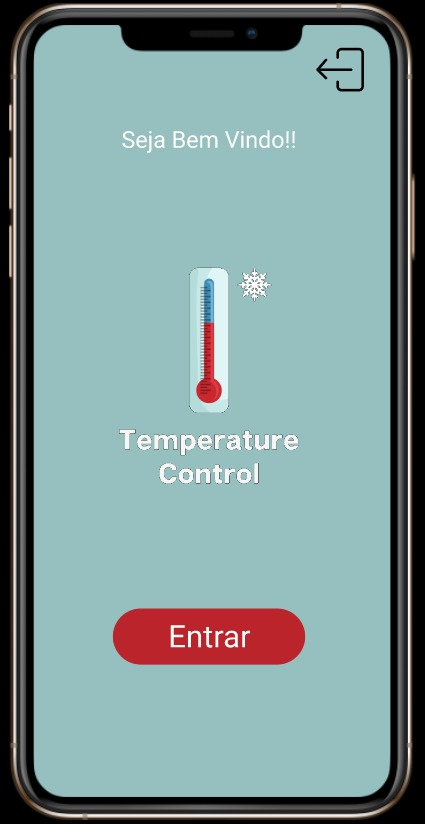
\includegraphics[scale=0.5]{img/mobile/bem_vindo.png}
        \legend{Fonte: Elaborado pelos autores}
        \label{fig:mobileBemVindo}
    \end{figure}

    \begin{figure}[ht]
        \caption{Layout mobile Home}
        \centering
        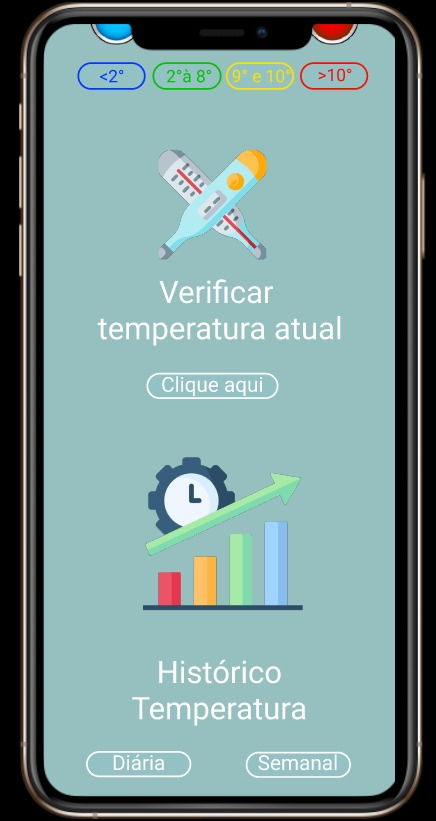
\includegraphics[scale=0.5]{img/mobile/home.jpeg}
        \legend{Fonte: Elaborado pelos autores}
        \label{fig:mobileHome}
    \end{figure}

    \begin{figure}[ht]
        \caption{Layout mobile configuração temperaturas}
        \centering
        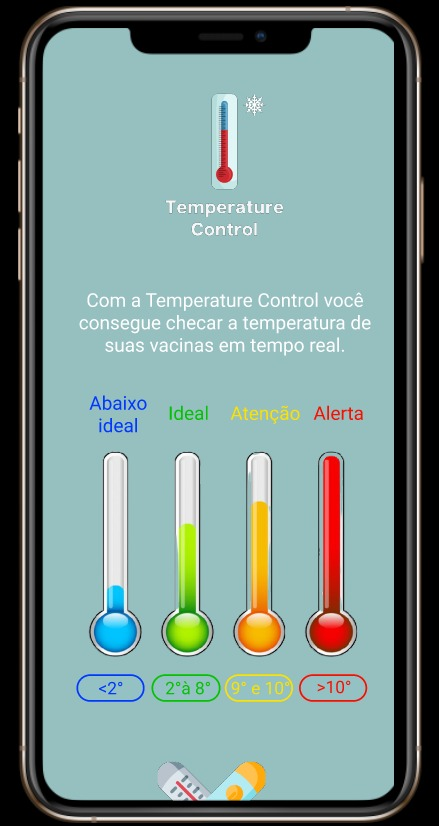
\includegraphics[scale=0.5]{img/mobile/config_temp.jpeg}
        \legend{Fonte: Elaborado pelos autores}
        \label{fig:mobileConfig}
    \end{figure}

    \begin{figure}[ht]
        \caption{Layout mobile dashboard 1}
        \centering
        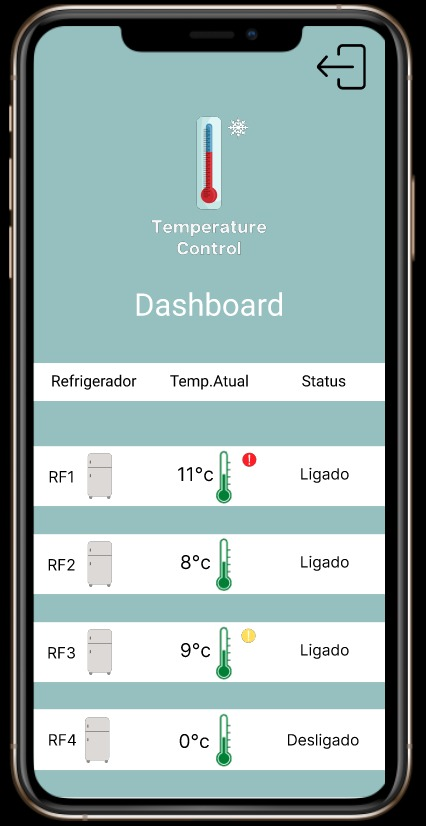
\includegraphics[scale=0.5]{img/mobile/dashboard_1.jpeg}
        \legend{Fonte: Elaborado pelos autores}
        \label{fig:mobileDashboard1}
    \end{figure}

    \begin{figure}[ht]
        \caption{Layout mobile dashboard 2}
        \centering
        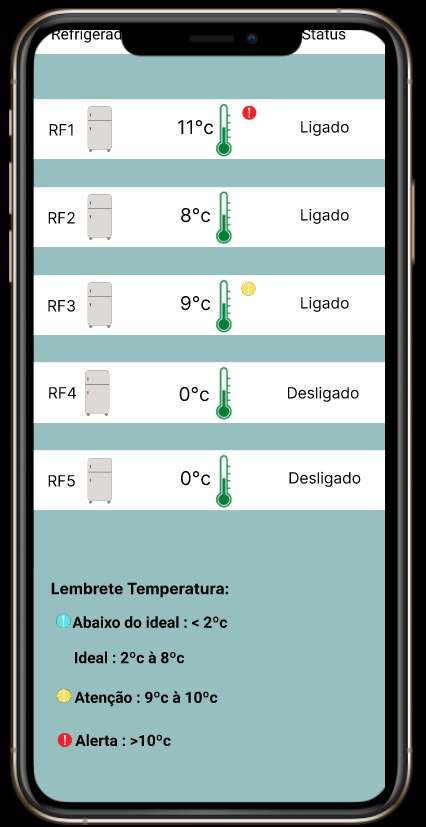
\includegraphics[scale=0.5]{img/mobile/dashboard_2.jpeg}
        \legend{Fonte: Elaborado pelos autores}
        \label{fig:mobileDashboard2}
    \end{figure}

    \begin{figure}[ht]
        \caption{Layout mobile temperatura atual}
        \centering
        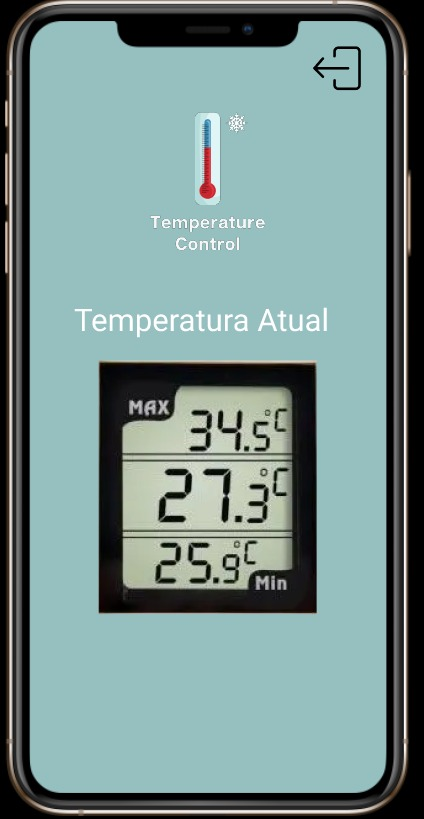
\includegraphics[scale=0.5]{img/mobile/temp_atual.jpeg}
        \legend{Fonte: Elaborado pelos autores}
        \label{fig:mobileTempAtual}
    \end{figure}

    \begin{figure}[ht]
        \caption{Layout mobile histórico diário}
        \centering
        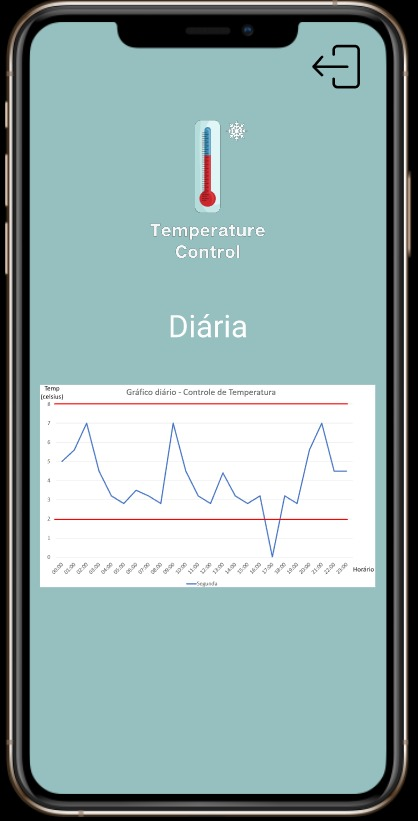
\includegraphics[scale=0.5]{img/mobile/temp_diaria.jpeg}
        \legend{Fonte: Elaborado pelos autores}
        \label{fig:mobileTempDiaria}
    \end{figure}

    \begin{figure}[ht]
        \caption{Layout mobile histórico semanal}
        \centering
        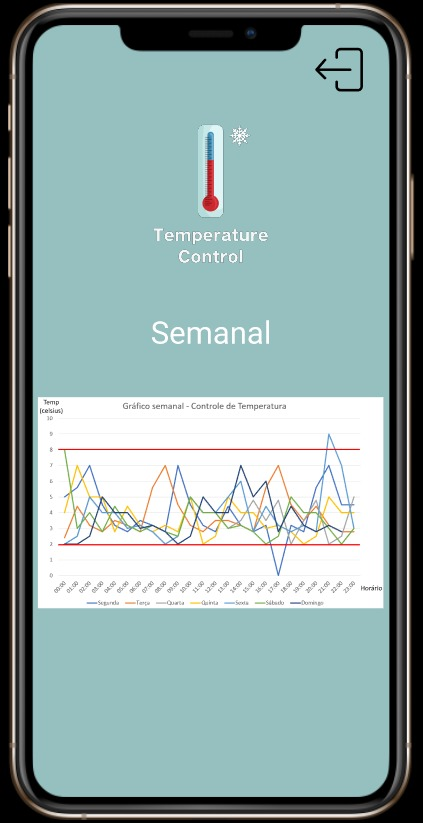
\includegraphics[scale=0.5]{img/mobile/temp_semanal.jpeg}
        \legend{Fonte: Elaborado pelos autores}
        \label{fig:mobileTempSemanal}
    \end{figure}


    % \begin{figure}[htb!]
        % \caption{Tela inicial do sistema}
        % \centering
        % 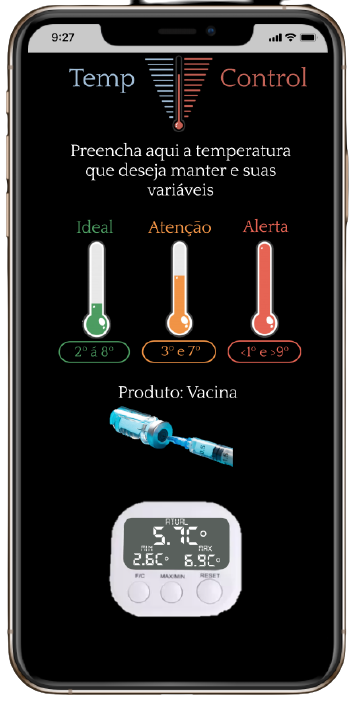
\includegraphics[scale=0.5]{img/sistema_home.png}
        % \legend{Fonte: Elaborado pelos autores}
        % \label{fig:sistemaHome}
    % \end{figure}
%
    % \begin{figure}[ht]
        % \caption{Tela de histórico de temperatura}
        % \centering
        % 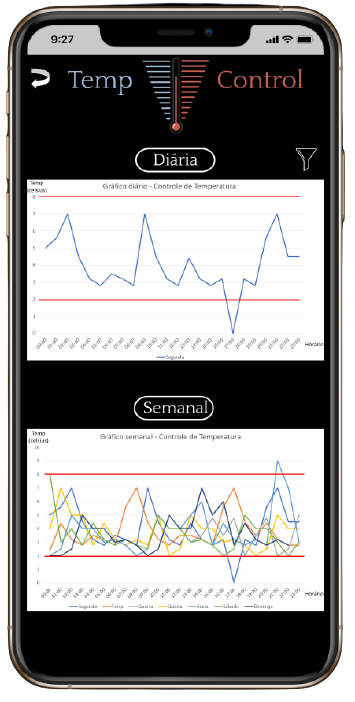
\includegraphics[scale=0.4]{img/sistema_historico.png}
        % \legend{Fonte: Elaborado pelos autores}
        % \label{fig:sistemaHistorico}
    % \end{figure}
%
    % \begin{figure}[t]
        % \caption{Tela de visualização em tempo real}
        % \centering
        % 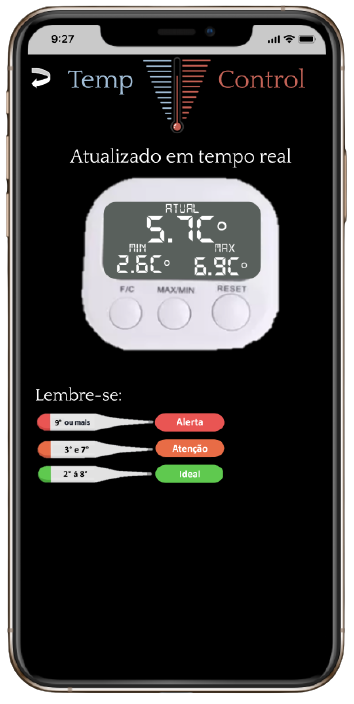
\includegraphics[scale=0.4]{img/sistema_temp_real.png}
        % \legend{Fonte: Elaborado pelos autores}
        % \label{fig:sistemaTempReal}
    % \end{figure}
%

    \begin{figure}[ht]
        \caption{Layout desktop home}
        \centering
        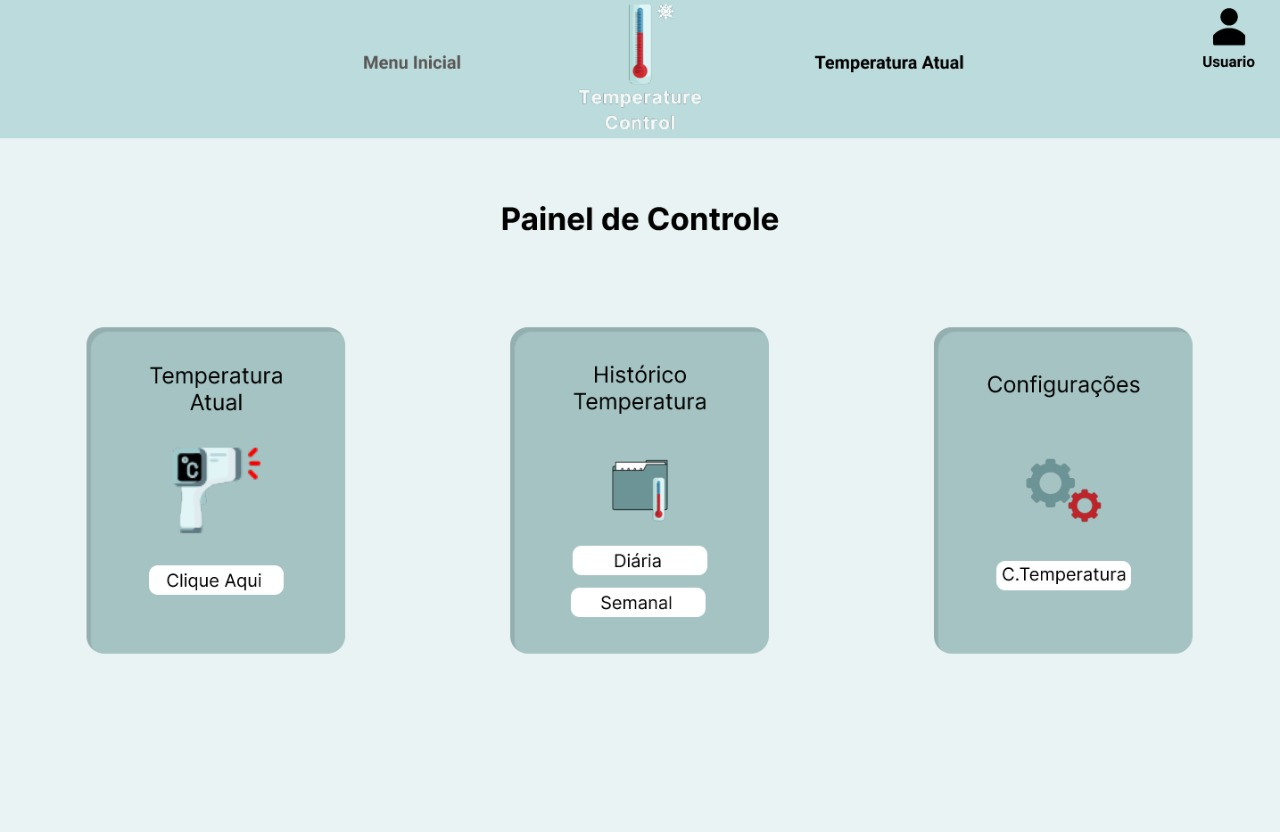
\includegraphics[scale=0.35]{img/desktop/home.jpeg}
        \legend{Fonte: Elaborado pelos autores}
        \label{fig:desktopHome}
    \end{figure}

    \begin{figure}[ht]
        \caption{Layout desktop configuração de temperatura}
        \centering
        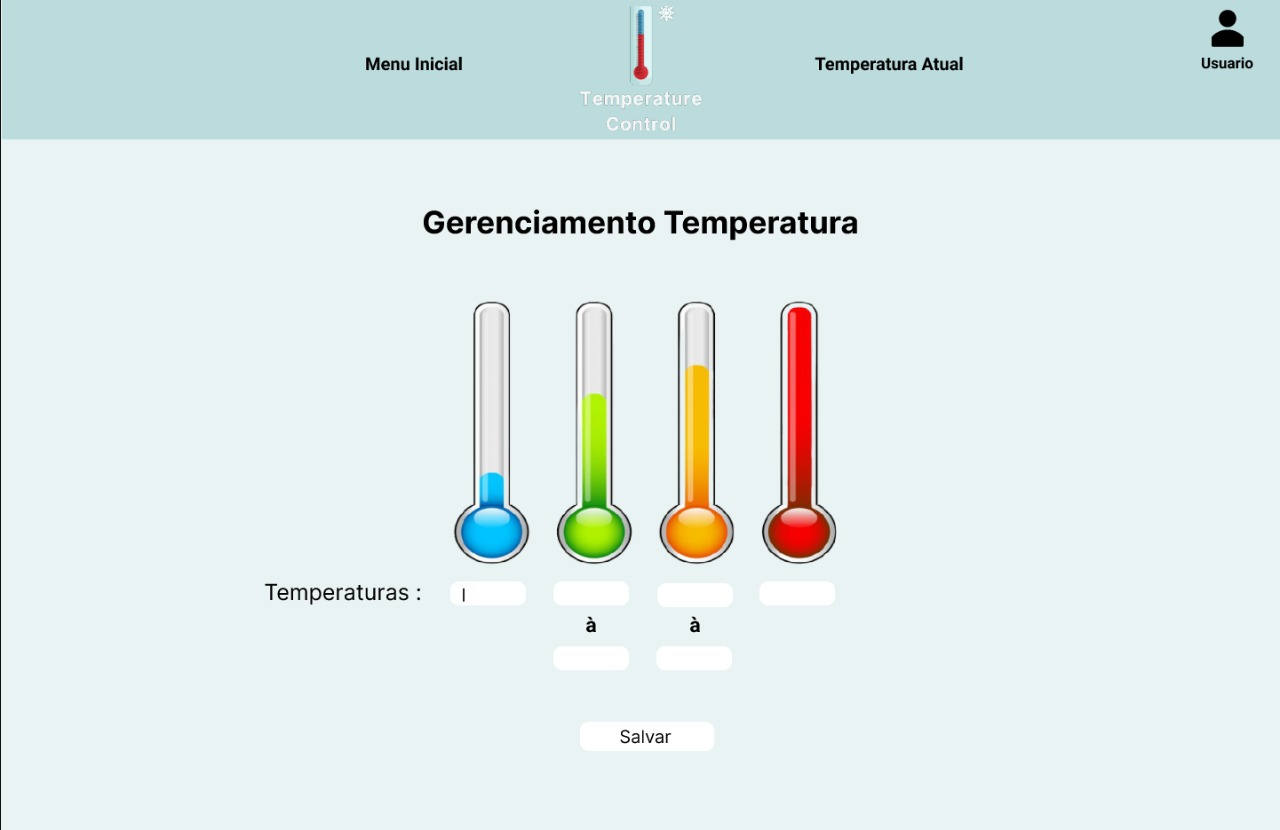
\includegraphics[scale=0.35]{img/desktop/config_temp.jpeg}
        \legend{Fonte: Elaborado pelos autores}
        \label{fig:desktopConfigTemp}
    \end{figure}

    \begin{figure}[ht]
        \caption{Layout desktop temperatura atual}
        \centering
        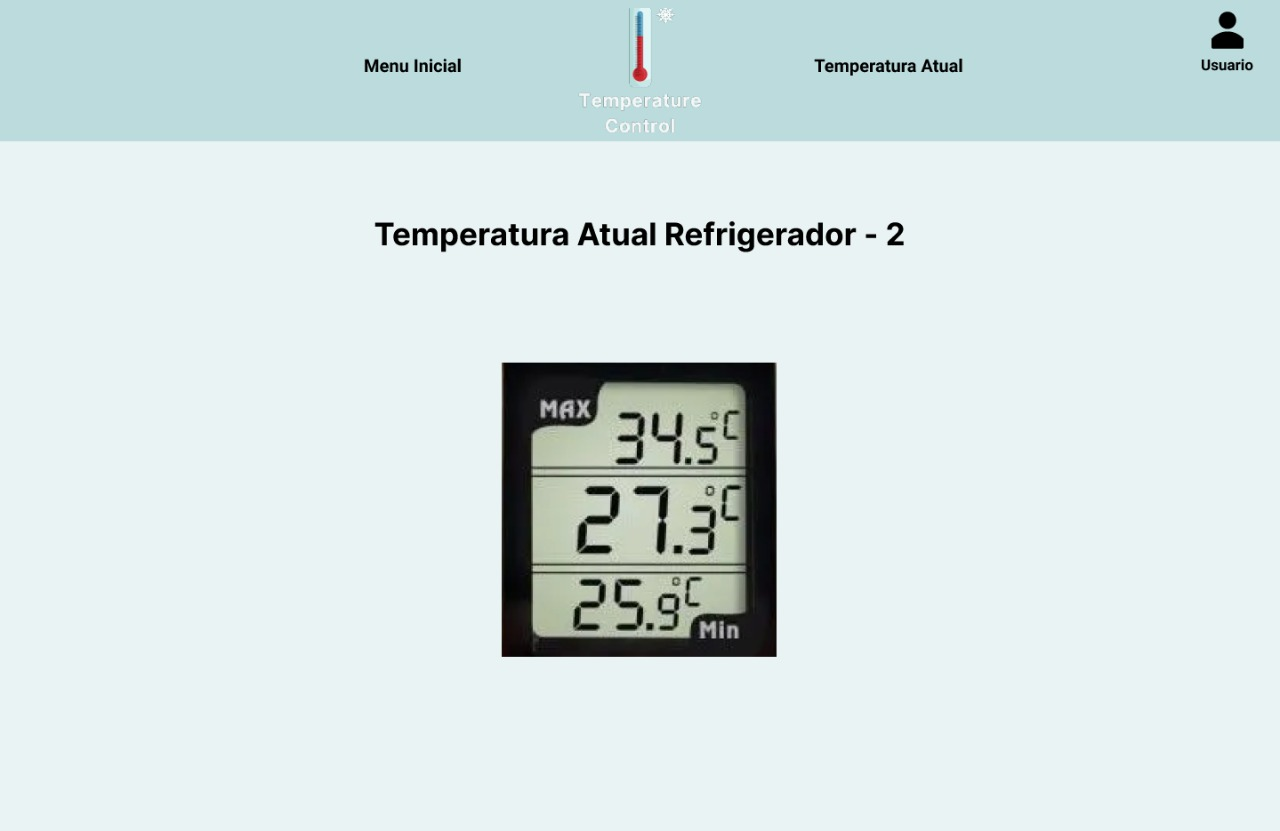
\includegraphics[scale=0.35]{img/desktop/temp_atual.jpeg}
        \legend{Fonte: Elaborado pelos autores}
        \label{fig:desktopTempAtual}
    \end{figure}

    \begin{figure}[ht]
        \caption{Layout desktop dashboard 1}
        \centering
        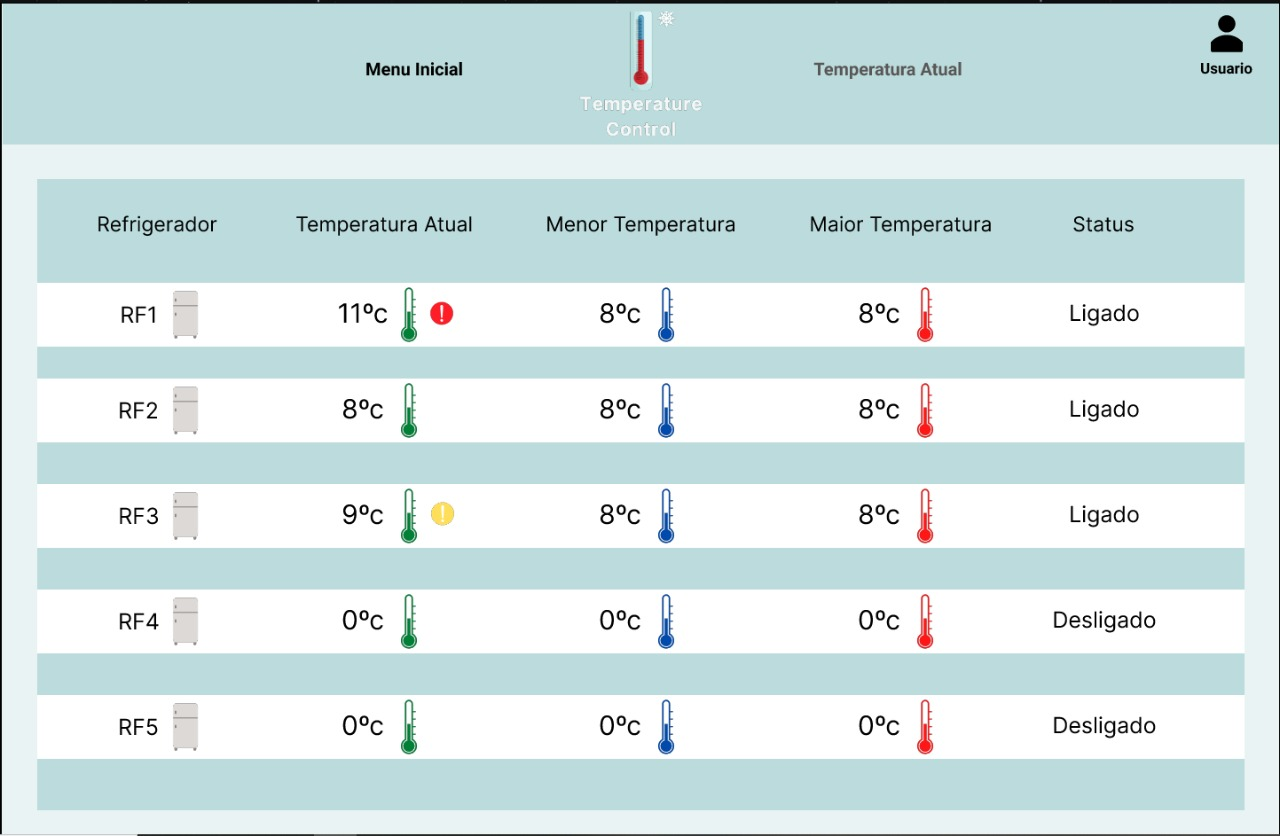
\includegraphics[scale=0.35]{img/desktop/dashboard_1.jpeg}
        \legend{Fonte: Elaborado pelos autores}
        \label{fig:desktopDashboard1}
    \end{figure}

    \begin{figure}[ht]
        \caption{Layout desktop dashboard 2}
        \centering
        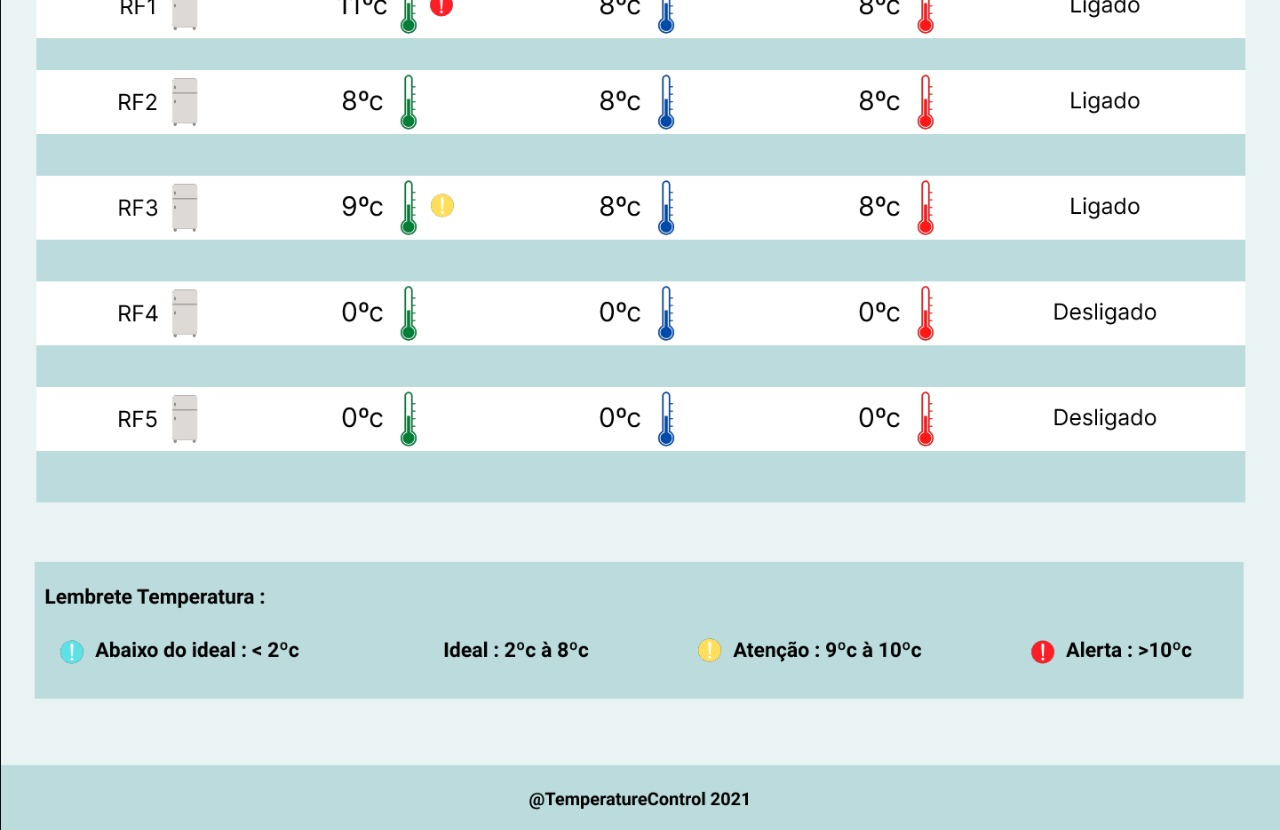
\includegraphics[scale=0.35]{img/desktop/dashboard_2.jpeg}
        \legend{Fonte: Elaborado pelos autores}
        \label{fig:desktopDashboard2}
    \end{figure}

    \begin{figure}[ht]
        \caption{Layout desktop histórico diário}
        \centering
        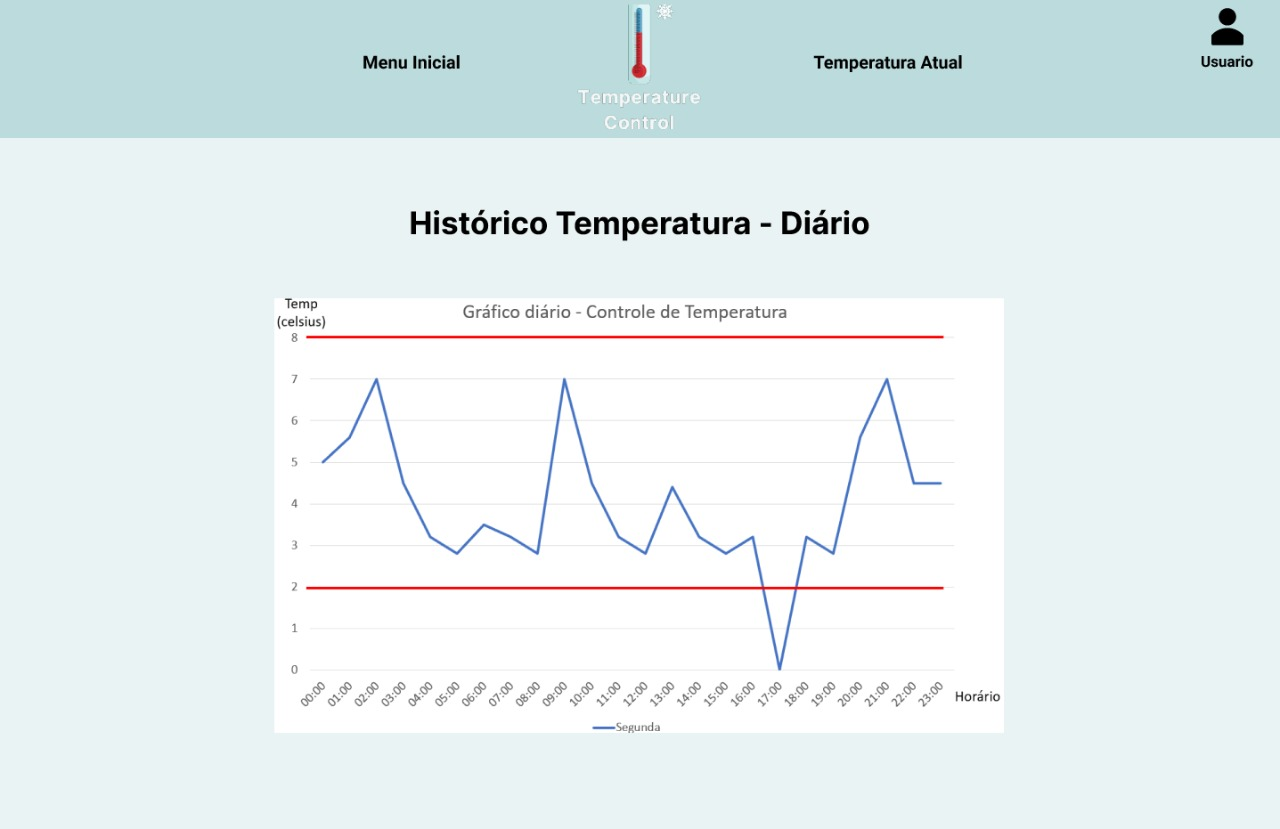
\includegraphics[scale=0.35]{img/desktop/temp_diaria.jpeg}
        \legend{Fonte: Elaborado pelos autores}
        \label{fig:desktopTempDiaria}
    \end{figure}

    \begin{figure}[ht]
        \caption{Layout desktop histórico semanal}
        \centering
        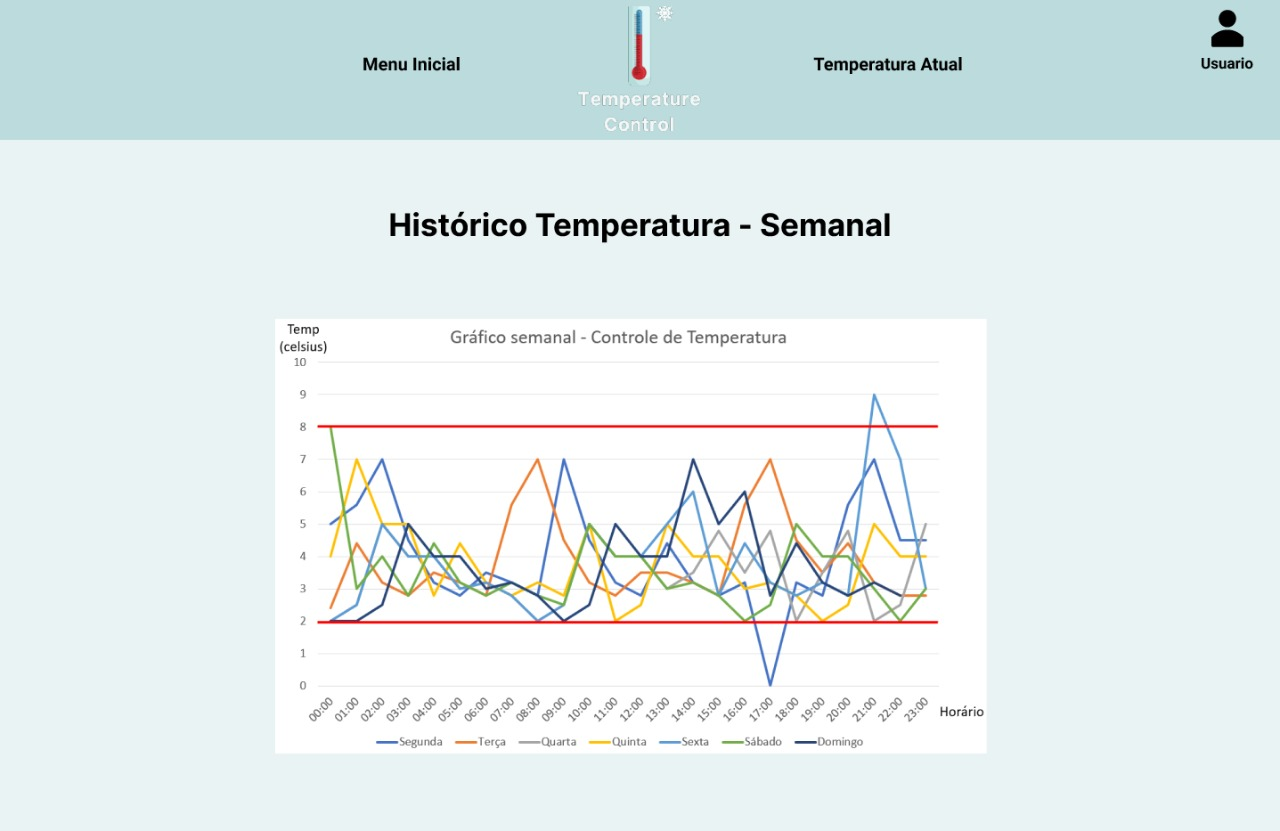
\includegraphics[scale=0.35]{img/desktop/temp_semanal.jpeg}
        \legend{Fonte: Elaborado pelos autores}
        \label{fig:desktopTempSemanal}
    \end{figure}


\chapter{Conclusão}

    Visando solucionar a demanda da empresa
    Rio Branco Alimentos SA/ Fábrica de Rações de Patrocínio
    da melhor forma possível cumpri-se todos os requisitos 
    por eles exigidos na descrição da demanda no Portal Saga SENAI
    foi idealizado esse projeto para de forma simples e eficaz 
    sanar as dores de nosso cliente.

    Para solucionar a demanda serão instalados sensores de 
    temperatura em cada freezer, bem como nas portas
    e assim poder informar os usuários sobre a temperatura
    interna das vacinas e emitir um alerta caso a temperatura
    saia de uma faixa predeterminada, normalmente de 2 a 8 ºC.

    Com o propósito de criar um histórico com as variações de 
    temperatura de cada freezer os dados de cada sensor de 
    temperatura serão transmitidos e guardados em um 
    banco de dados que poderá ser consultado a qualquer momento
    pelos usuários, também será possível visualizar a temperatura
    em tempo real de cada freezer e receber alerta e notificações
    caso a temperatura saia do nível esperado.

    Com esse projeto escrito pelos autores 
    será possível evitar várias perdas de vacinas por 
    falta de gerenciamento da temperatura dos freezeres
    em que as mesmas são guardadas, além de gerar maior valor 
    agregado ao processo e ao produto, garantindo 
    a qualidade e a confiabilidade das vacinas.

    \begin{figure}
        \caption{Canvas}
        \centering
        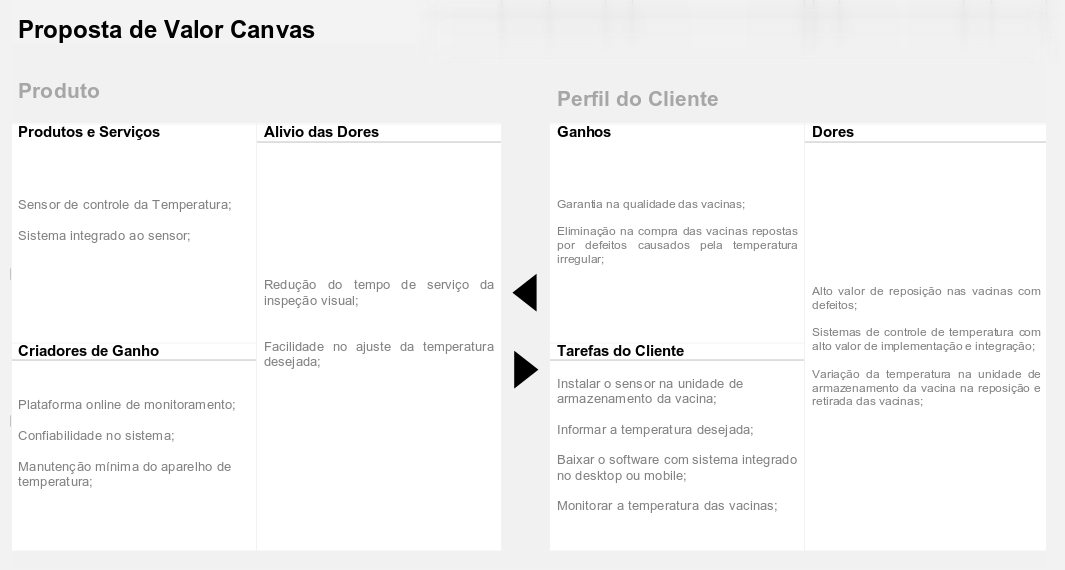
\includegraphics[width=0.9\textwidth]{img/canvas.png}
        \legend{Fonte: Elaborado pelos autores}
        \label{fig:canvas}
    \end{figure}


\postextual

\bibliography{referencias}

\end{document}
